\clearpage
\section{Historical Overview of Code Generation by LLMs}

The history of code generation can be explored from several 
perspectives. 

\subsection{Natural Language Processing} %%%%%%%%%%%%%%%%%%%%%%%%%%%%%
One possible starting point for 
analysing the evolution of code generation is to trace
the development of Natural Language Processing (NLP), 
the field that studies how machines process and interact 
with human language. NLP comprises two major subdomains: 
Natural Language Understanding (NLU), which focuses on a 
machine's ability to interpret and "understand" human language, 
and Natural Language Generation (NLG), which concerns the 
generation of natural-sounding text.

This distinction is particularly relevant because 
the technologies currently used for code generation 
are essentially the same as those employed for natural 
language generation. In fact, Transformer-based models 
trained on source code data approach code generation in 
the same way they would handle natural text generation 
by predicting sequences of tokens in context using learned 
statistical patterns \cite{vaswani2017attention}.

From this point of view, the starting point can be traced back to 1943, 
during World War II, with the invention of Colossus, one of the first digital 
electronic computers, developed to analyse encrypted communications from the 
German military

In parallel, the discipline of Natural Language Processing 
(NLP) began to take shape as early as the 1940s, culminating 
in the 1954 Georgetown experiment the first public demonstration 
of machine translation. Another milestone came in 1966 with the 
creation of ELIZA \cite{weizenbaum1966eliza}, considered the first 
chatbot in history, which simulated the behaviour of a psychotherapist 
using pattern-matching rules.

During the 1970s and 1980s, symbolic approaches to NLP became popular. 
These early attempts aimed to enable machines to “understand” language 
through manually encoded rules and logic-based systems. In the 1990s, 
the importance of statistical methods became evident, marking a shift 
from rule-based to probabilistic models for language processing.

In 2006 Google launched its now ubiquitous Google 
Translate service. The following decade saw the rise of voice-based 
assistants: Apple’s Siri (2011), Microsoft’s Cortana (2014), 
Amazon’s Alexa (2014), and Google Assistant (2016).

A major breakthrough came with the introduction of distributed word 
representations, especially word2vec \cite{mikolov2013efficient} and 
GloVe \cite{pennington2014glove}, published in 2013 and 2014 respectively. 
These methods enabled dense vector representations that captured semantic 
relationships between words in large corpora.

The most significant leap, however, occurred in 2017 with the publication 
of the now seminal paper “Attention is All You Need” 
\cite{vaswani2017attention}, which introduced the Transformer 
architecture. This architecture remains the dominant framework in 
NLP and underpins nearly all modern LLMs. Transformers enabled major 
advances in tasks such as text generation, machine translation, 
question answering, text summarization and, more recently, code 
generation.

The first LLMs capable of code generation began to appear around 
2019–2020, notably with the release of GPT-2 \cite{radford2019language}. 
In 2021, OpenAI released Codex \cite{chen2021codex}, a GPT-3 \cite{brown2020language} derivative 
trained specifically for code generation and explanation, which was
later integrated into GitHub Copilot.

Between 2022 and 2024, a wave of new LLMs for code generation was 
released, including CodeT5 \cite{wang2021codet5}, CodeGen 
\cite{nijkamp2022codegen}, CodeGeeX \cite{zeng2022codegeex}, 
and Code LLaMA \cite{roziere2023code}.


\subsection{Code Generator} %%%%%%%%%%%%%%%%%%%%%%%%%%%%%
\label{sec:Code_Generator}
Fortran is a 
programming language with an integrated compiler, developed by IBM. 
A compiler can be seen as a code generation tool, since it 
translates source code into machine code, the only “language” 
truly “understandable” by a computer \cite{backus1957fortran}.

Compilers have a long history and have been continuously 
improved over time, but they are not the only tools for code 
generation. Already in 1976, the concept of intelligent editors 
emerged with Emacs, thanks to its support for custom macros 
\cite{stallman1981emacs}. Later, in 1996, IntelliSense 
introduced symbolic completion, namely the ability of the IDE 
to suggest code based on the context and the symbols already present.

In 1999, with XSLT, one of the first standardized tools for 
automatic transformation between markup languages was introduced 
\cite{xslt1999}. During the same years, the work of Zelle\cite{zelle1996learning}
and  Mooney\cite{mooney1997nlidb} (1996–1999) 
proposed methods based on Natural Language 
processing to generate database queries from natural language 
expressions.

At the same time, template-engine-based tools  for server-side 
spread, such as Jinja2 (2005)\cite{jinja2docs} 
and Mako (2006)\cite{makoengine}, 
was developed the generation of 
dynamic code by combining data with predefined structures. 

In 2017, with research on AST-guided code generation, LSTM 
models began to be used to generate code in a more structured 
way, guided by the syntax of the programming language 
\cite{yin2017syntactic}.

In 2021 GitHub Copilot, one of the most advanced 
code completion tools was introduced: so efficient that it is 
capable of generating entire code sections from simple textual 
prompts, thanks to the use of generative AI models based on 
Transformer architectures \cite{chen2021codex}.




\subsection{LLMs code oriented} %%%%%%%%%%%%%%%%%%%%%%%%%%%%%
The publication of the 
paper \textit{Attention Is All You Need} \cite{vaswani2017attention} 
in 2017, which 
introduced the Transformer architecture, 
enabled the widespread development of
Large Language Models (LLMs). 
It should be noted that the first LLMs were typically designed 
to analyse and generate only natural language text, so not all LLMs 
were capable of generating code, or at least of generating syntactically 
correct or functional code.

In 2018, two foundational models were introduced: BERT 
\cite{devlin2019bert}, an encoder-only architecture 
designed to generate dense semantic representations of 
natural language, and GPT-1 \cite{radford2018improving}, 
a decoder-only model capable of generating coherent text. 
Those models were not yet able to generate code, but they have been 
an important baseline for future code-oriented models.

In fact in 2019, OpenAI released GPT-2 \cite{radford2019language}, 
a more powerful decoder-only model capable of producing much 
more convincing text compared to GPT-1. Although GPT-2 was 
not specifically trained to generate code, its training 
corpus included code snippets. In the same year, 
TabNine, a popular code completion extension for several IDEs, 
replaced its n-gram-based next-token prediction with a version 
of GPT-2 fine-tuned on source code \cite{tabnine2019}.

Also in 2019, Microsoft Research and GitHub introduced the 
CodeSearchNet dataset \cite{husain2019codesearchnet}, a 
multilingual code dataset and one of the first large-scale 
corpora usable to train Transformers for code generation tasks.

In 2020, Microsoft Research released CodeBERT 
\cite{feng2020codebert} \textit{(based on BERT)}, 
trained on both natural 
language and code using the CodeSearchNet dataset. 
CodeBERT is designed for tasks such as code search 
and code summarization. While it does not generate code, 
it is an encoder-only model capable of deeply understanding 
the structure and semantics of source code. Through 
CodeBERT is possible producing rich 
and dense representations suitable for downstream tasks like 
classification, or for use as input to decoders in generative 
pipelines.

In 2021, several LLMs capable of generating realistic and 
reliable code were introduced. OpenAI published Codex 
\cite{chen2021codex}, a GPT-3 \cite{brown2020language} derivative fine-tuned on 
source code from the GitHub Code dataset. In the same paper 
OpenAI introduced the HumanEval benchmark, designed to assess the 
performance of Codex \cite{chen2021codex} on programming problems 
\textit{(and in future all LLMs code oriented)}.
On HumanEval, Codex (12B) was able to solve 28.8\% 
of the problems on the 
first attempt, significantly outperforming all previous 
models on code generation.

Codex \cite{chen2021codex} sparked widespread interest in the use of LLMs 
for code generation, indeed in the same year it was released 
GitHub Copilot, powered by Codex \cite{chen2021codex}.

In the same year, 
many additional datasets were 
published, including MBPP (Mostly Basic Python Problems) 
\cite{austin2021program}, the APPS dataset \cite{hendrycks2021measuring}, 
and CodeXGLUE \cite{lu2021codexglue}.

In December 2021, Salesforce AI Research released CodeT5 
\cite{wang2021codet5}, an open-source encoder-decoder 
model that, unlike Codex \cite{chen2021codex}, supports a wider variety of 
code-related tasks. Thanks to task-specific training strategies, 
CodeT5 proved to be highly versatile, supporting code 
summarization, generation, and translation.

In 2022, Google introduced AlphaCode \cite{li2022competition}, 
achieving a performance in the top 54.3 percentile on 
competitive programming tasks on Codeforces. In the same 
year, PolyCoder \cite{xu2022systematic}, a decoder-only 
model trained solely on 249 GB of source code, was also 
released as an open-source alternative. 

In 2023, GPT-4 \cite{openai2023gpt4} (although not 
exclusively trained for code generation)  
achieved an 80\% success rate on HumanEval. 
Claude 3 by Anthropic reportedly reached 85\%, 
and Meta’s open-source model Code LLaMA 
\cite{roziere2023code} scored 57\%.

In 2024, Google introduced Gemini \cite{AlphaCode_2}, 
which, when integrated into an inspired AlphaCode framework, 
reached performance within the top 15\% of coding competition 
participants.



\begin{figure}[ht]
    \centering
    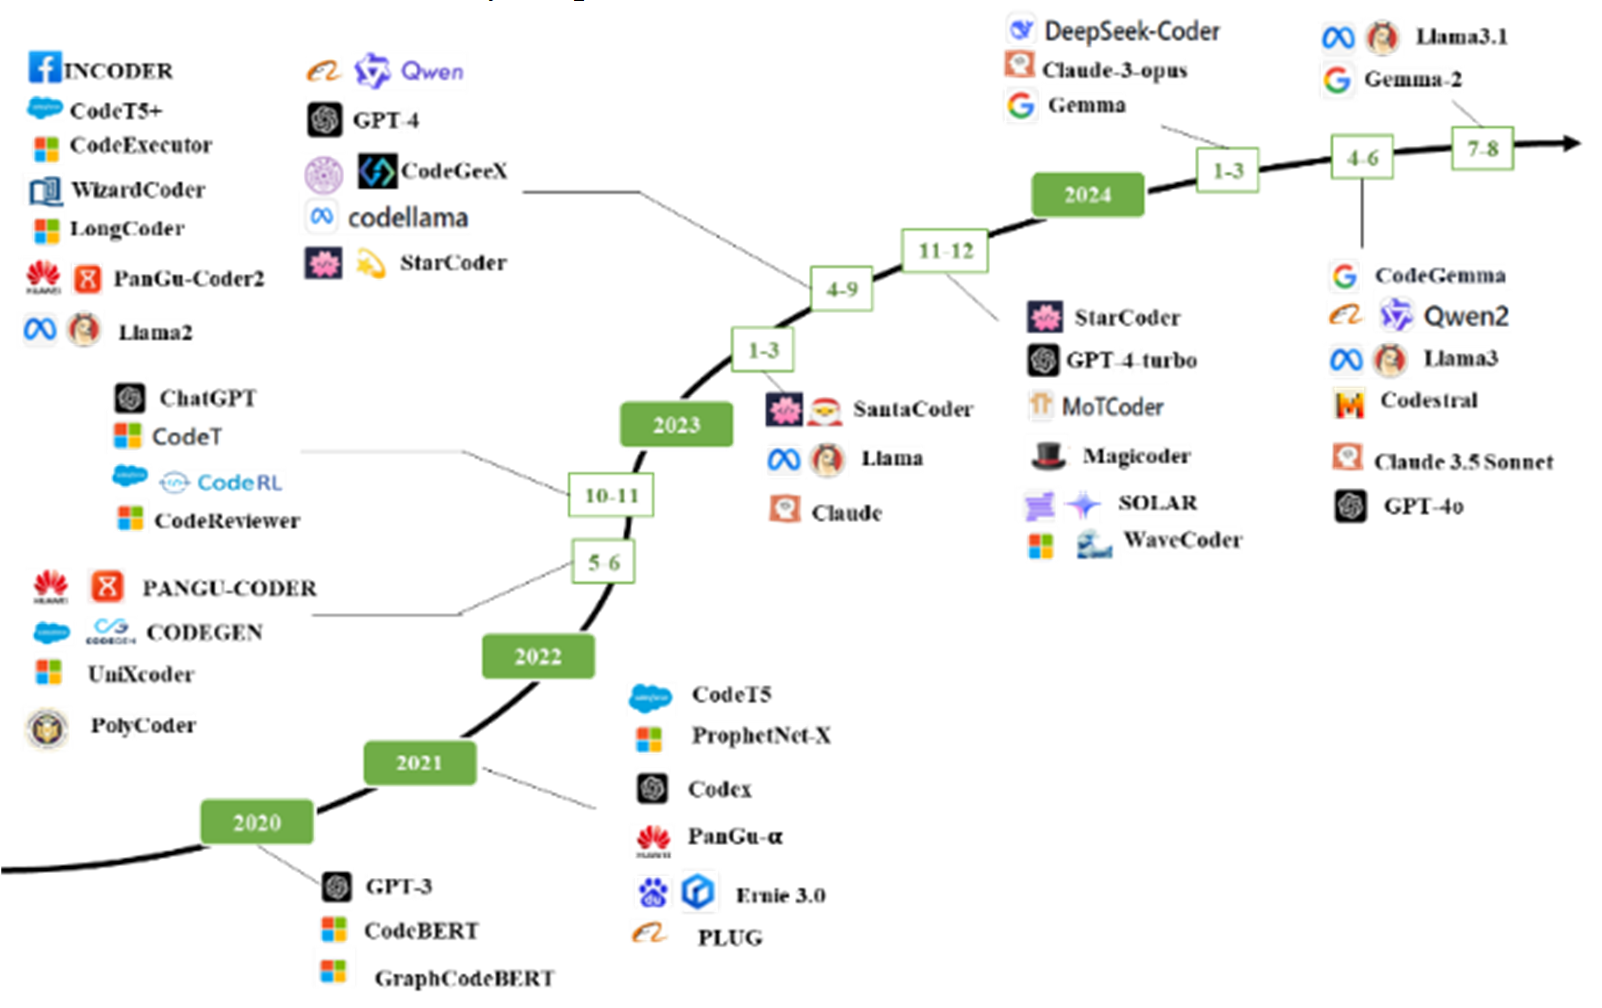
\includegraphics[width=0.8\textwidth]{img/CodeGenerator.png}
    \caption{Timeline of code generation by LLM \cite{wu2022research}.}
    \label{fig:LLM-coder-examples}
\end{figure}